% --- COMMANDS ---
\makeatletter
\define@key{entry}{sound}[]{\def\entry@sound{#1}}
\define@key{entry}{pos}[]{\def\entry@pos{#1}}
\define@key{entry}{etym}[]{\def\entry@etym{#1}}
\define@key{entry}{note}[]{\def\entry@note{#1}}

\setkeys{entry}{sound,pos,etym,note}

\newcommand{\entry}[3][]{%
\begingroup%
\setcounter{sense}{1}%
\setkeys{entry}{#1}%
\par \begin{minipage}{\columnwidth}%
	\textbf{\rzc #2}%
	\ifdefempty{\entry@pos}{}{ • {\footnotesize\it\entry@pos}}%
	\ifdefempty{\entry@sound}{}{ • {\footnotesize\entry@sound}}%
	\ifdefempty{\entry@etym}{}{ ← {\footnotesize\entry@etym}}%
	\ifdefempty{\entry@note}{}{ • {\footnotesize\entry@note}}%
	\ • #3%
\end{minipage}%
\endgroup%
}

\newcounter{sense}
\NewDocumentCommand{\sense}{o}{%
\ifnum\the\value{sense}>1 \fi%
	\textbf{\arabic{sense}} %
	\IfNoValueTF{#1}{}{\ {#1}}%
\stepcounter{sense}%
}

\makeatother

\setchapterpreamble[u]{\margintoc}
\chapter{Lexicon}
A \langname{}-to-English dictionary is provided below.

\section*{How to use}
Entries for lexical items are listed by their spelling in generic form, ignoring morphophonological alterations. Derived words are listed as separate entries, but their source word is given. On the other hand, idiomatic or fixed expressions are given under the lexical item.

Each sense of a word has three basic parts: a quick, single-word translation for ease-of-use; a more detailed explanation of the concept; and an example sentence. The sentences are usually designed to help the reader figure the word's meaning out from context, particularly for \langname{} speakers and learners.

Pronunciations are given dictionary-style in a phonetic alphabet more intuitive to native \langname{} speakers. See §\ref{ch:segments} for more about the sounds of \langname{} and their transcriptions.

\pagelayout{wide}
\setlength{\columnsep}{30pt}
\begin{multicols}{2}

\addsec{A}
\entry[pos=prn.]{a}{\sense second-person pronoun }
\entry[pos=noun]{adahę́s}{\sense sand \sense[(idiom)] citizens \sense[(\rzc\bf z-adahę́s)] public, people }
\entry[pos=prep.]{ah}{\sense at }
\entry[pos=noun]{ahka}{\sense pair of feet \sense[(\rzc\bf ahka mei)] foot \sense wisdom \sense[(adj., of people)] wise \sense[(adj., of things)] trusty, reliable \sense[(\rzc\bf ahka esyi)] aphorism }
\entry[pos=verb in.,etym=\rz{ahka} + -m]{ahkam}{\sense journey to \rz{tę} }
\entry[pos=verb tr.,etym=\rz{husal} + -\rz{eks}]{akral}{\sense give \sense[(refl.)] hold, own \sense leads to, correlates with }
\entry[sound=/akvo/,pos=noun]{akva}{\sense valley }
\entry[pos=noun]{almani}{\sense wave \sense current, riptide }
\entry[pos=noun]{as}{\sense foreigner }
\entry[pos=noun]{atlar}{\sense ceremonial cord \sense police \sense police officer }
\entry[sound=/áttę̆l/,pos=verb tr.]{attąl}{\sense sift, sort through: \rz{sec attęssi siazr t-makra m-mas t-kiray nahó séc} “he combed the sand for an hour trying to find his ring” \sense collect, pile together: \rz{sec attęssi nahazŕ t-hels m-het} “he collected the rings together into a mountain” }
\entry[pos=verb tr.]{azyam}{\sense[(of crops)] plant, sow \sense[(idiom, of people)] give birth to }

\addsec{Ą}
\entry[pos=verb tr.]{ąk}{\sense eat }
\entry[pos=adj.]{ąs}{\sense wet }

\addsec{B}
\entry[pos=verb tr.]{bęssat}{\sense perform a dance with \rz{u} someone: \rz{sec bąsseci yésacza u-mans husalaks} “he's performed the two step with famous people” }

\addsec{C}
\entry[sound=/círĕ/,pos=noun]{cira}{\sense salad: \rz{rat otr partedal s-ąk cira, tęlr rat ócaa hetr} “I'm thinking of eating salads to get thin” }
\entry[pos=noun]{cǫhi}{\sense undershirt, underwear \sense dress }
\entry[sound=/cózzĕ/,pos=noun]{cozza}{\sense pole \sense[(adj., of people)] sober \sense[(adj., of things)] rigid, firm }
\entry[pos=noun]{cunna}{\sense medium sized seawater fish \sense[(\rzc\bf cunna retus)] river fish \sense[(\rzc\bf cunna lǫya)] small fish \sense[(\rzc\bf cunna ócaa)] eel, oarfish \sense[(\rzc\bf cunna sapa)] shark }

\addsec{E}
\entry[pos=noun]{ecma}{\sense wool, linen }
\entry[pos=noun]{ecmalǫya}{\sense pants \sense shoes }
\entry[pos=ptcl.]{egi}{\sense just, only }
\entry[pos=noun]{emassoi}{\sense boss \sense coach, manager \sense[(\rzc\bf emassoi kąstezi)] on-field coach \sense[(\rzc\bf emassoi ǫkas)] general manager }
\entry[sound=/émăs/,pos=noun]{ems}{\sense[(ntr.)] plot of land }
\entry[pos=noun]{ens}{\sense[(ntr.)] in, inner \sense[(adj.)] inner }
\entry[pos=verb tr.,etym=\rz{ens} + \rz{sat}]{ensat}{\sense approach }
\entry[pos=verb tr.]{ensel}{\sense help with \rz{im} }
\entry[pos=adj.]{esyi}{\sense good \sense correct, appropriate }
\entry[pos=prep.]{ez}{\sense among, in \sense made of }
\entry[pos=prep.]{ezzu}{\sense associates of }

\addsec{G}
\entry[pos=noun]{gelaǫ́}{\sense[(ntr.)] fort \sense college, university }
\entry[pos=noun]{gerraós}{\sense a man's given name }

\addsec{H}
\entry[pos=noun]{hakra}{\sense battle, skirmish \sense[(pl.)] military campaign \sense[(pl., of school)] semester }
\entry[sound=/hĕlíŏ/,pos=noun]{halia}{\sense body part \sense[(\rzc\bf halia ąs)] internal organ }
\entry[pos=noun]{halma}{\sense[(of distance)] far}
\entry[sound=/hą́nĕ/,pos=noun]{hąna}{\sense coil \sense length of rope or wire \sense[(adj., of people)] drunk: \rz{emassoin m-rat ikuci retą s-ot hąna rat} “our boss bought shots and I got drunk” }
\entry[sound=/hŏriamázi/,pos=noun]{hariamazi}{\sense weaver, embroider, seamstress \sense[(\rzc\bf hariamazi men)] tailor }
\entry[sound=/hŏssúsăl/,pos=verb tr.]{hassusal}{\sense exalt, praise \sense[(refl.)] boast about \rz{tę} \sense root for, cheer for }
\entry[sound=/hélas/,pos=noun]{hels}{\sense[(ntr.)] mountain }
\entry[pos=noun]{hemza}{\sense big cat }
\entry[pos=verb in.]{het}{\sense be at: \rz{sec h-tesa heci} “he's at the beach” }
\entry[pos=noun]{hora}{\sense wrist \sense[(idiom)] craftmanship, handiness: \rz{hakra sec pici} “he's talented” }
\entry[sound=/hórǫ̆kăs/,pos=noun]{hórąks}{\sense mathematics }
\entry[pos=noun]{horiama}{\sense weaving, embroidery }
\entry[pos=verb tr.]{husal}{\sense shout at }
\entry[pos=noun]{husaleks}{\sense[(ntr.)] fame \sense[(adj.)] famous }

\addsec{I}
\entry[pos=noun]{iama}{\sense knot \sense[(adj.)] woven }
\entry[pos=noun]{iamac}{\sense[(ntr.)] webbing, netting \sense displeasing pattern \sense chaos: \rz{paknan oci t-iamac h-makra m-piran} “the kids turned the chose into chaos” }
\entry[pos=verb tr.]{ikut}{\sense buy }
\entry[pos=prep.]{im}{\sense of \sense from }
\entry[pos=noun]{ista}{\sense[(ntr.)] decaffenated tea \sense[(adj., of coffee)] decaf \sense[(adj., of alcohol)] virgin \sense[(religious)] grace, a quite prayer for blessing food or travel }
\entry[pos=noun]{isyus}{\sense[(ntr.)] shield \sense special forces }

\addsec{K}
\entry[sound=/kĕgę́să/,pos=noun]{kagęsa}{\sense army \sense[(of sports)] team, club }
\entry[pos=ptcl.]{kai}{\sense says, saying }
\entry[pos=noun]{kams}{\sense back, the part of the body opposite the face below the neck and above the thigh, including the buttocks \sense[(\rzc\bf t-kams im)] after }
\entry[pos=noun]{kemu}{\sense fruit slice }
\entry[pos=noun]{kęsa}{\sense soldier \sense[(of literature)] protagonist, hero }
\entry[pos=noun]{kę́samen}{\sense fashion police }
\entry[sound=/kę́stĕt/,pos=verb tr.]{kęstat}{\sense lead towards \rz{tę} a goal \sense command: \rz{nassoin kateci s-kągęsa s-kagę́staspa} “the king commands both army and navy” \sense train in \rz{tę} a skill: \rz{t-horam iama kąstetri rat lala} “auntie's teaching me to sew” \sense formally school in \rz{ez} a discipline: \rz{rappahan pici kąstettal z-latya} “the minister was brought up in the faith” }
\entry[pos=noun]{kęstatvassa}{\sense pioneer, trendsetter }
\entry[pos=noun]{kipira}{\sense teenager }
\entry[pos=verb tr.]{kiray}{\sense search for \sense find }
\entry[sound=/kotŏssói/,pos=noun]{kotassoi}{\sense[(of people)] body, self }
\entry[pos=noun]{kotus}{\sense[(ntr.)] divinity \sense[(adj.)] divine }

\addsec{L}
\entry[pos=noun]{laczi}{\sense faith }
\entry[pos=noun]{lala}{\sense auntie }
\entry[pos=noun]{lar}{\sense something, anything }
\entry[pos=noun]{latta}{\sense paella, a seafood dish served over grains }
\entry[pos=noun]{layac}{\sense religious ministry \sense college, university }
\entry[pos=verb in.]{lǫit}{\sense run }
\entry[pos=noun]{lǫya}{\sense shin, the part of the body above the foot and below the thigh, including the knee and upper ankle }

\addsec{M}
\entry[pos=noun]{makra}{\sense shoulder \sense responsibility, duty \sense[(adj., of people)] mature, responsible \sense[(\rzc\bf h-makra im)] because of, due to \sense[(\rzc\bf sat makra)] resolve, become decisive \sense[(\rzc\bf ems makra)] leader, person in charge \sense[(\rzc\bf hels makra)] foundation }
\entry[pos=noun]{mana}{\sense coffee }
\entry[pos=noun]{mans}{\sense[(ntr.)] somebody, anybody }
\entry[pos=noun]{mas}{\sense[(ntr.)] hour }
\entry[pos=noun]{mazzi}{\sense ballplayer }
\entry[pos=noun]{meatrę́}{\sense[(ntr., medical)] body part, limb: \rz{sec rakés meatrę́ aczá h-makra m-kęsa m-ot} “he lost two limbs as a soldier” \sense[({\rzc\bf meatrę́ ens}, ntr., medical)] internal organ }
\entry[pos=noun]{men}{\sense[(ntr.)] over, outer \sense[(adj.)] outer \sense jacket, shirt \sense clothing }
\entry[pos=noun]{ménhakra}{\sense gear, equipment: \rz{kąsazr het sedal t-kęstat t-uthet ménhakra sec} “soldiers must be trained to clean their equipment” \sense[(fashion)] accessory \sense[(\rzc\bf ménhakra secya)] hat, visor, hood }
\entry[pos=noun]{meniama}{\sense shirt }
\entry[pos=noun]{ménisyus}{\sense body armor \sense[(adj.)] armored, fortified: \rz{yiazin parseci tasaklá menisyús} “the thief stole the armored truck” }
\entry[pos=noun]{ménsapr}{\sense coat, jacket }
\entry[pos=verb tr.]{mensat}{\sense leave }
\entry[pos=noun]{meva}{\sense house cat }
\entry[pos=noun]{miyi}{\sense nose \sense bravery \sense[(adj., of people)] heroic: \rz{nassoin miyin kąsteci Katva z-dahę́s t-hakra} “the heroic king lead the Katva people into battle” }
\entry[pos=prn.]{moc}{\sense third-person pronoun for neuter gender }
\entry[sound=/mósĕt/,pos=verb tr.]{mosat}{\sense[(of things)] to lose, to cede, to have taken from }
\entry[pos=noun]{mulkas}{\sense[(ntr.)] fur, pelt \sense[(ntr., of people)] body hair }

\addsec{N}
\entry[pos=noun]{naha}{\sense hoop, ring }
\entry[pos=noun]{nahozzi}{\sense hooper, \rz{táhątnaha} player }
\entry[pos=noun]{nassoi}{\sense king }

\addsec{O}
\entry[sound=/ócoa/,pos=adj.]{ócaa}{\sense deep \sense[(of people)] tall and wiry }
\entry[pos=noun]{ocza}{\sense two }
\entry[sound=/orra/,pos=adj.]{orra}{\sense dry \sense[(of food)] stale \sense[(of people)] feeble, frail \sense[(of things)] subpar, fragile }
\entry[pos=verb in.]{ossat}{\sense grow \sense[(of people)] develop emotionally }
\entry[]{ot}{}
\entry[pos=verb in.]{ot}{\sense be: \rz{kęsa sec oci} “he's a soldier” \sense[(\rzc\bf ot tę)] become }

\addsec{Ǫ}
\entry[sound=/ǫ́kăs/,pos=noun]{ǫks}{\sense[(ntr.)] payment }

\addsec{P}
\entry[pos=noun]{pakna}{\sense house }
\entry[pos=noun]{páknalac}{\sense[(ntr.)] inn, motel, short-term lodgings for a traveller between urban areas }
\entry[pos=noun]{palac}{\sense[(ntr.)] dinner }
\entry[pos=noun]{parsa}{\sense eyes }
\entry[pos=noun,etym=\rz{parsa} + \rz{iamac}]{parsiamac}{\sense hallucination }
\entry[pos=noun]{patla}{\sense cold \sense[(\rzc\bf z-patla het)] be cold \sense[(\rzc\bf patla yat)] it's cold }
\entry[pos=noun]{pava}{\sense family }
\entry[pos=noun]{pira}{\sense child }
\entry[pos=verb in.]{pit}{\sense have: \rz{meniaman sec pici} “it's his shirt” }
\entry[pos=verb tr.]{porsat}{\sense[(of high value items)] rob, steal }
\entry[sound=/pórtĕm/,pos=verb tr.]{portam}{\sense dance with: \rz{kipiran partemsi mans tevi z-layac} “that guy danced with almost everybody at the college” \sense try on, try out: \rz{rappahan partemsi ménsapr sova} “the minister's trying out a new coat” \sense taste: \rz{rat semr t-portam latczŕ husaléks} “I might try the renowned paella” \sense consider: \rz{rat portag s-kęstat lala} “I'm thinking of hiring a nanny” \sense[(science)] conduct an experiment: \rz{sec portamés mens ocaa m-akral sonza m-táhątnaha} “I've heard they're studying how height correlates to tag talent” }
\entry[pos=noun]{purrés}{\sense a woman's given name }

\addsec{R}
\entry[pos=noun]{rappaha}{\sense minister }
\entry[sound=/ráprę/,pos=noun]{raprą}{\sense ore, raw metal }
\entry[pos=noun]{raprę́}{\sense[(ntr.)] car, truck \sense[({\rzc\bf raprę́ ócaa}, ntr.)] bus: \rz{atlar kęstac rapręzr ócaa z-kams m-ǫkas esyi} “the police operate buses at a fair price” \sense[({\rzc\bf raprę́ hemza} ntr.)] motorbike \sense[({\rzc\bf raprę́ meva} ntr.)] moped }
\entry[sound=/rĕsrę́/,pos=noun]{rasrę́}{\sense[(ntr.)] webbing, netting \sense pleasing pattern \sense[(music)] harmonious }
\entry[pos=prn.]{rat}{\sense first-person pronoun }
\entry[sound=/retosat/,pos=verb tr.,etym=\rz{reta} "sharp" + -t]{ratosat}{\sense cut, slice \sense cross through }
\entry[sound=/retǫ̆/,pos=noun]{retą}{\sense punch, hit \sense shot of alcohol or tea }
\entry[pos=verb tr.]{rǫssat}{\sense meet \sense[(school)] begin to learn, start to learn }
\entry[pos=verb in.]{ruhum}{\sense[(of animals)] bark, yelp }

\addsec{S}
\entry[pos=noun]{sapatesa}{\sense change of opinion \sense[({\rzc\bf sat sapatesa}, informal)] do a 180 on \rz{tę} something: \rz{nassoin saci sapatesa t-kęstat vącizr} “the king changed his mind on hiring mercenary bands” }
\entry[pos=noun]{sapa}{\sense hunt \sense dog }
\entry[pos=noun]{sapr}{\sense fur }
\entry[pos=verb tr.]{sat}{\sense go to \sense do }
\entry[pos=noun]{sąttis}{\sense leafy green }
\entry[pos=verb in.]{sayenar}{\sense be ignorant about \rz{ez} }
\entry[pos=prn.]{sec}{\sense third-person pronoun for common gender }
\entry[pos=noun]{secya}{\sense celestial object, sun, moon, star \sense[\rzc\bf t-secya] today }
\entry[pos=verb tr.]{sem}{\sense say to, talk to \sense talk to about \rz{ez} \sense speak on, discuss \sense[(\rzc\bf sem véaja)] preach about \rz{ez} \sense[(refl.)] say \sense want someone to \rz{im} do \sense want to \rz{su} do \sense[(\rzc\bf sem tę)] should, ought to, hopefully will \sense[(\rzc\bf segi te)] let's do, let's go to \sense[(of words)] signify, mean, be defined as \sense[(of titles)] enable, allow to \sense[(informal)] looks like }
\entry[pos=noun]{sia}{\sense sand }
\entry[pos=ptcl.]{solr}{\sense and }
\entry[pos=noun]{sonza}{\sense tree branch \sense skill, natural talent }
\entry[pos=adj.]{sova}{\sense new }
\entry[pos=prep.]{su}{\sense and }

\addsec{T}
\entry[sound=/táhę̆t/,pos=verb in.]{tahąt}{\sense[(of people)] stretch \sense reach for \rz{tę} \sense pray about \rz{ez} }
\entry[pos=noun]{táhątnaha}{\sense tag, a parkour game played on an obstalce cours between two teams trying to grab rings to score 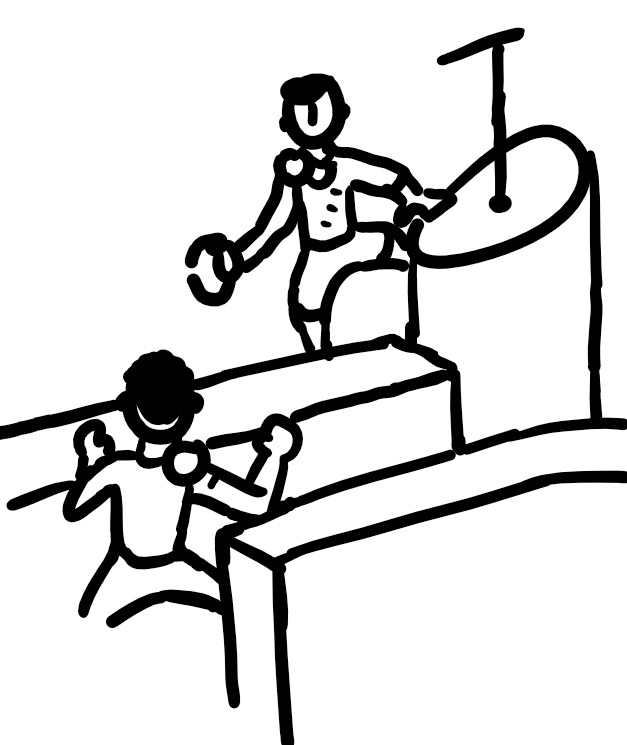
\includegraphics[width=\columnwidth]{sisik.png} }
\entry[sound=/tĕsísyŏ/,pos=noun,etym=\rz{tesa} + \rz{isyo}]{tasisya}{\sense city \sense port }
\entry[pos=noun]{taspa}{\sense sea \sense country }
\entry[pos=prep.]{tę}{\sense to \sense from }
\entry[pos=ptcl.]{tęlr}{\sense thus, therefore \sense[(discourse)] anyways... }
\entry[pos=noun]{tesa}{\sense shore, beach }
\entry[sound=/tăsékla/,pos=noun]{tsekla}{\sense rein \sense steering wheel \sense[(informal)] truck, car }

\addsec{U}
\entry[pos=prep.]{u}{\sense with \sense and }
\entry[pos=verb tr.]{uthet}{\sense clean }

\addsec{V}
\entry[pos=noun]{vassa}{\sense tide \sense[(idiom)] important moment }
\entry[pos=noun]{vęci}{\sense mercenary }
\entry[pos=noun]{vekkar}{\sense[(ntr.)] set, collection \sense[(adj., of things)] complete, whole \sense[(adj., of people)] organized }
\entry[sound=/vézŏm/,pos=verb in.]{vezam}{\sense accept, agree to \rz{ez} }

\addsec{Y}
\entry[pos=noun]{yar}{\sense[(ntr.)] year }
\entry[pos=verb in.]{yat}{\sense[(of weather)] occur, happen }
\entry[pos=noun]{yésacza}{\sense two step, a very basic line dance easily learned }
\entry[pos=noun]{yesi}{\sense foot step }
\entry[pos=verb tr.]{yiat}{\sense[(of low value items)] steal, nab, }
\entry[pos=noun]{yiatyar}{\sense timesink }
\entry[pos=noun]{yiazi}{\sense thief }
\entry[pos=noun]{yira}{\sense a type of flower that grows on the river bed \sense[(name)] a male given name }

\addsec{Z}
\entry[pos=noun]{zalmi}{\sense the sun \sense[(\rzc\bf t-zalmi)] tomorrow }
\entry[pos=noun]{ząsta}{\sense vine nut }

\end{multicols}